\documentclass[a4,12pt]{article}

% 畫圖
\usepackage{tikz}
\usetikzlibrary{automata,positioning,arrows}


% 排版
% \usepackage{enumerate}
% \newlist{steps}{enumerate}{1}
% \setlist[steps, 1]{label = Step \arabic*:}

% 中文插件
\usepackage{fontspec}
\usepackage{xeCJK}
\setCJKmainfont{Heiti TC}


% 插入圖片 using \includegraphics[scale = 1]{name.jpg}
\usepackage{graphicx}
\graphicspath{{./picture/}}
\usepackage{float} %设置图片浮动位置的宏包
\usepackage{subfigure}

% \usepackage[]{caption}
% \capto

\usepackage{multicol}

\title{Computer Graphics Hw 2} 
\author{賴柏勛 00957126}

\begin{document}
    \maketitle
    \section{操作方法}

    W、S:按住可以前後走。

    A、D:旋轉。

    R、F:當靠近可拾取物品時,分別可以用左手或右手來拾取物品。
    
    J:平凡無奇的跳。

    O:變成 orz 模式。
    \section{設計}
        由於 glut 鍵盤的 callback function 觸發速度過慢,如果我想將走路、旋轉變的流暢,
        就不能使用每次觸發移動一次的方式,因此我鍵盤 callback function 只會刷新我走路的時間並加速,在這樣的方式下,
        我走路的速度會帶有加速度並且看起來比鍵盤觸發的還流暢。

        根據以上原則,我其他的動作也遵循這個方式,因此速度不會被 glut callback 的速度限制住,但是也戳到了一些之前沒有想到的東西,
        例如當物件變多時,由於我的動作被 display 的速度限制,因此每個動作的速率都被拖慢,
        下次如果還要實作的話,應該會嘗試使用其他計數器\(例:time.h 的  clock\_gettime\)來計算動作所需要的時間。
        
    \section{scene graph}   

    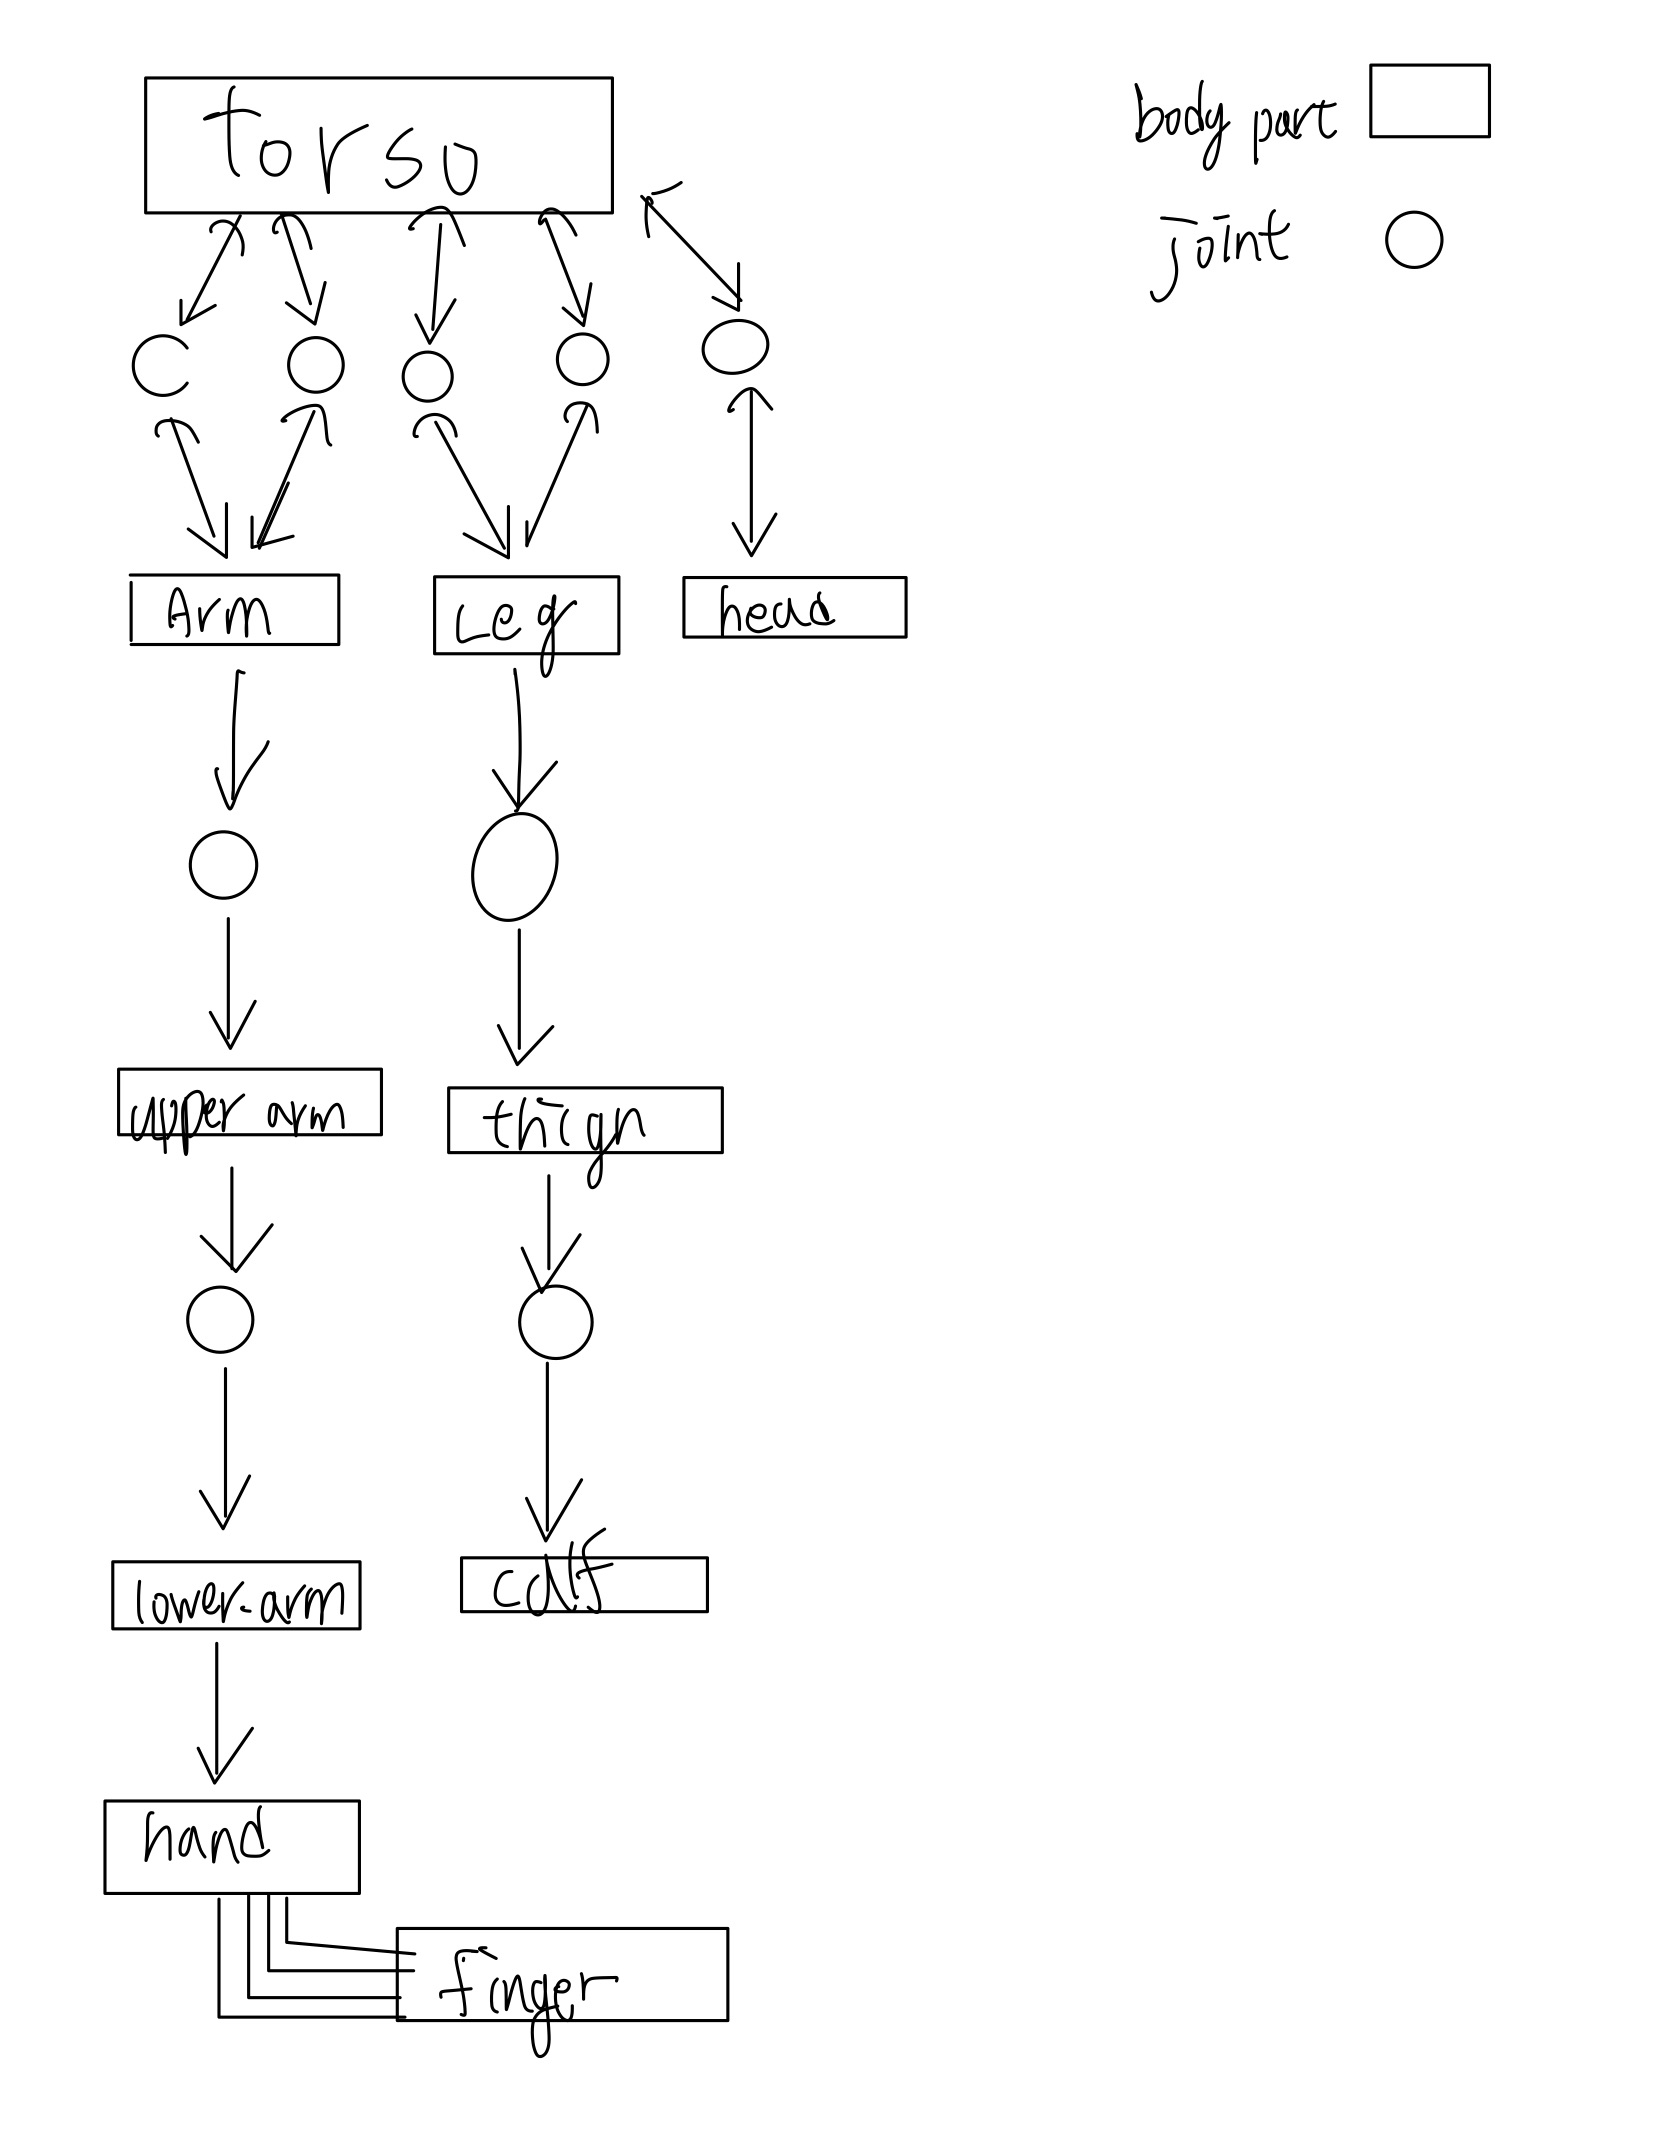
\includegraphics[scale=0.3]{scene_graph.jpg} 
    \section{實機畫面}
    \begin{figure}[H] 
    \centering
    
    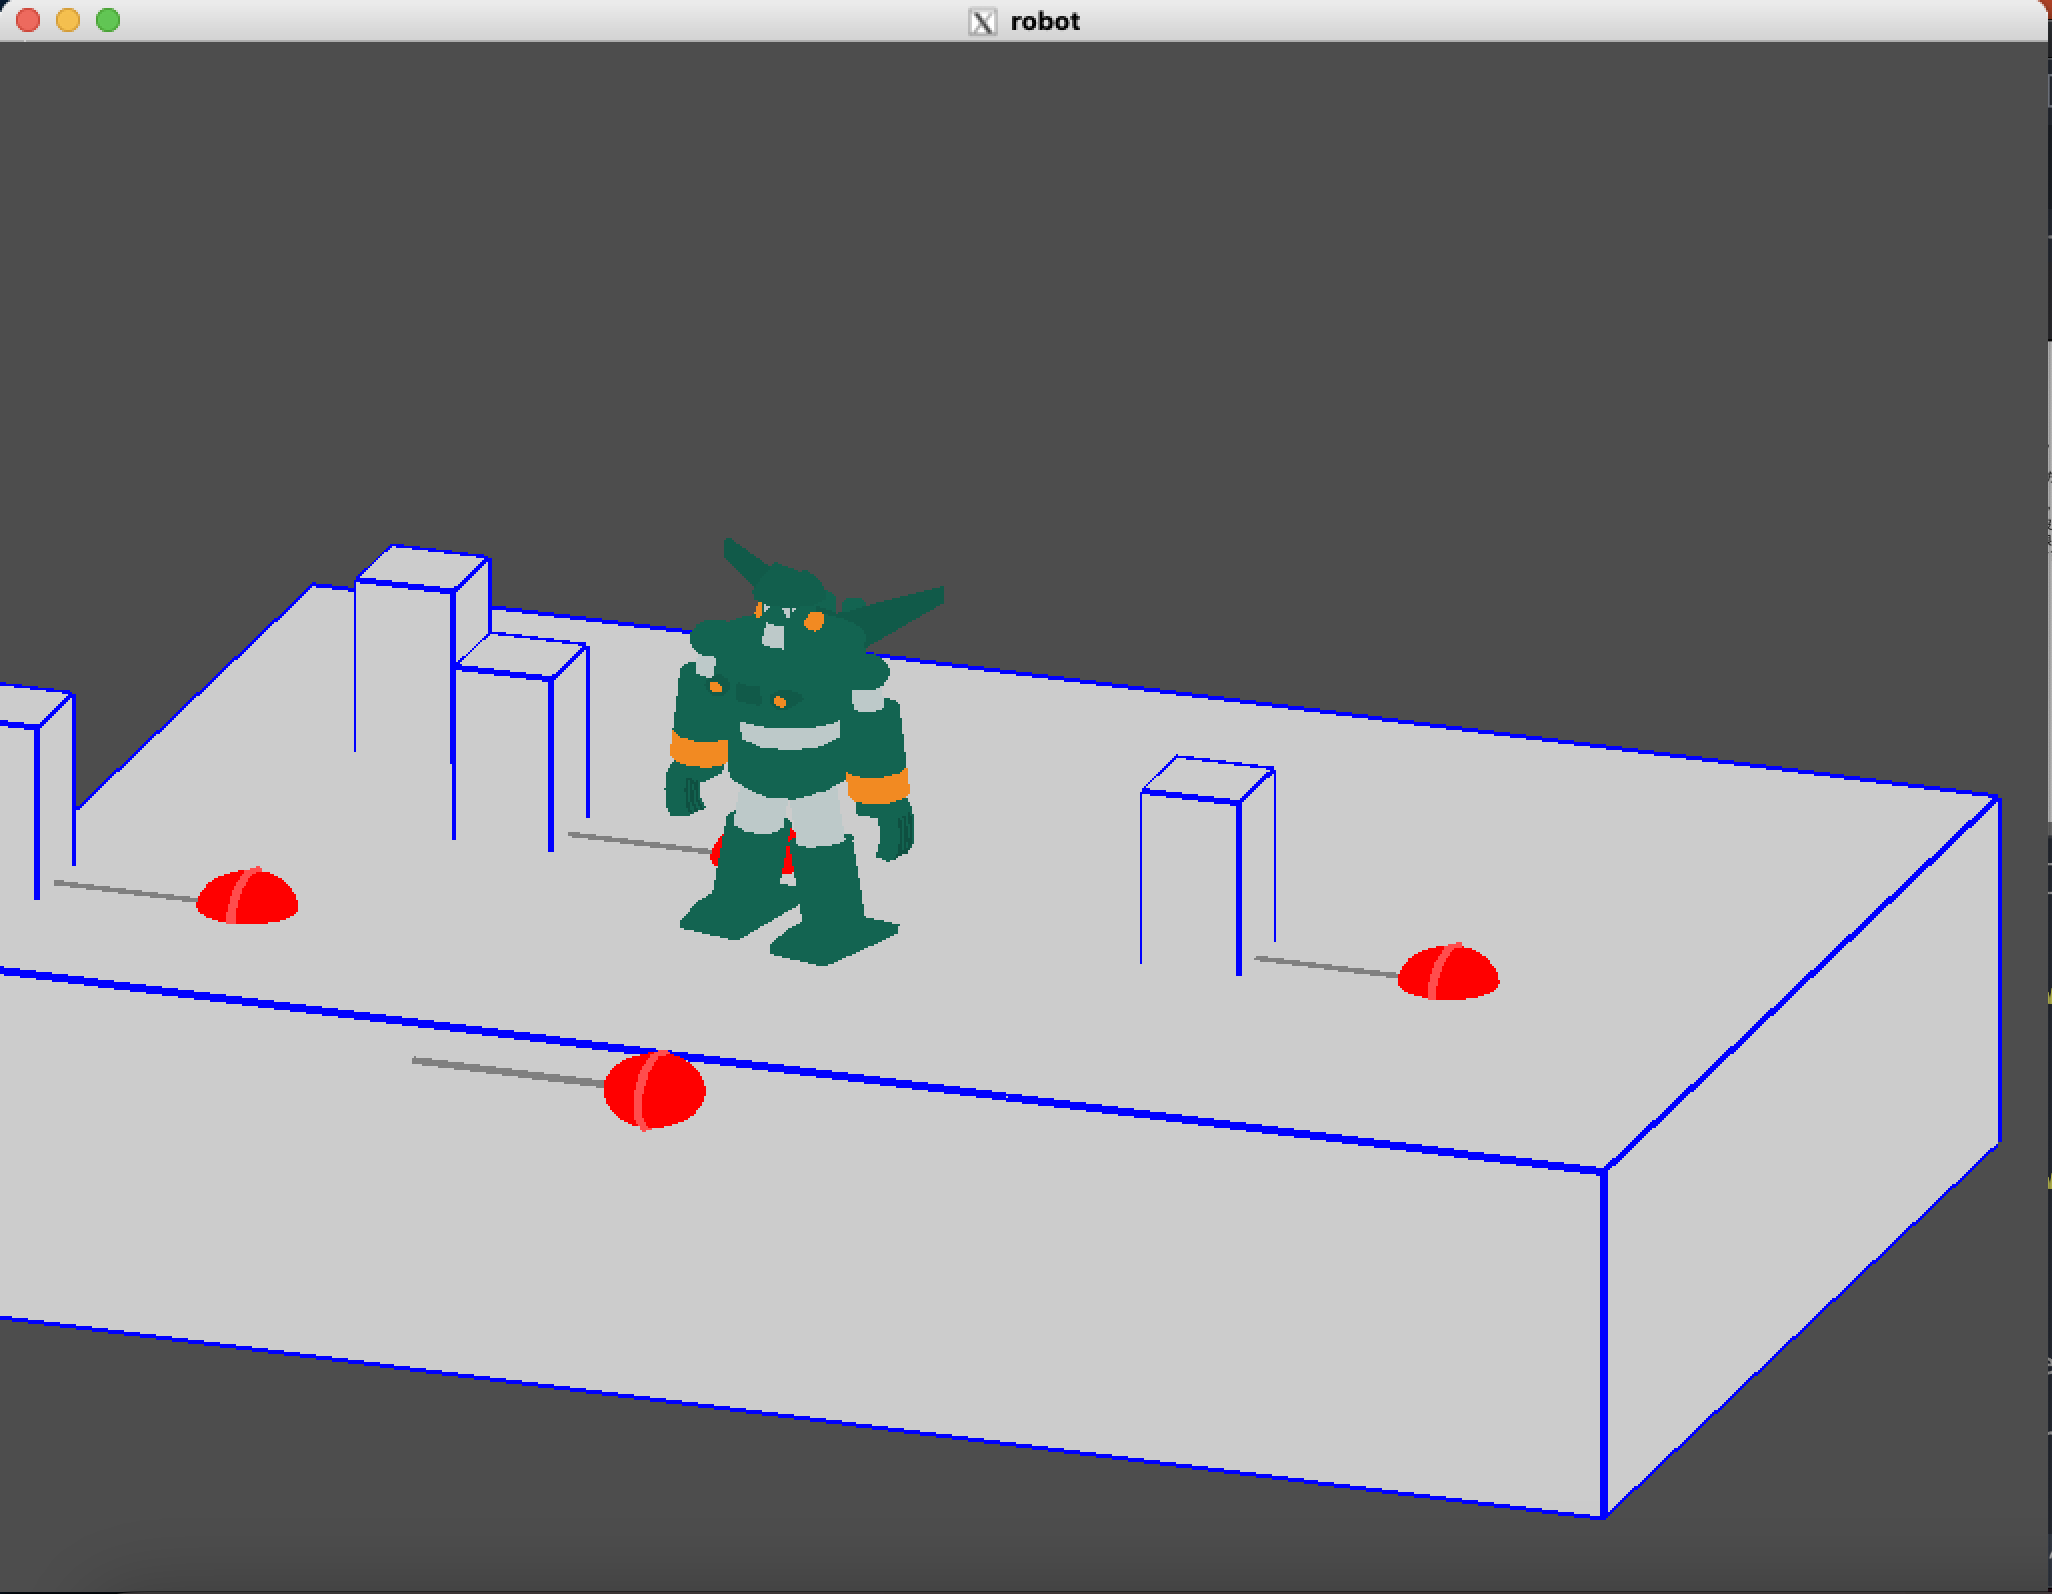
\includegraphics[scale = 0.3]{robot1.png}
    \caption{機器人}
    \end{figure}
    \begin{figure}[H] 
        \centering
       
    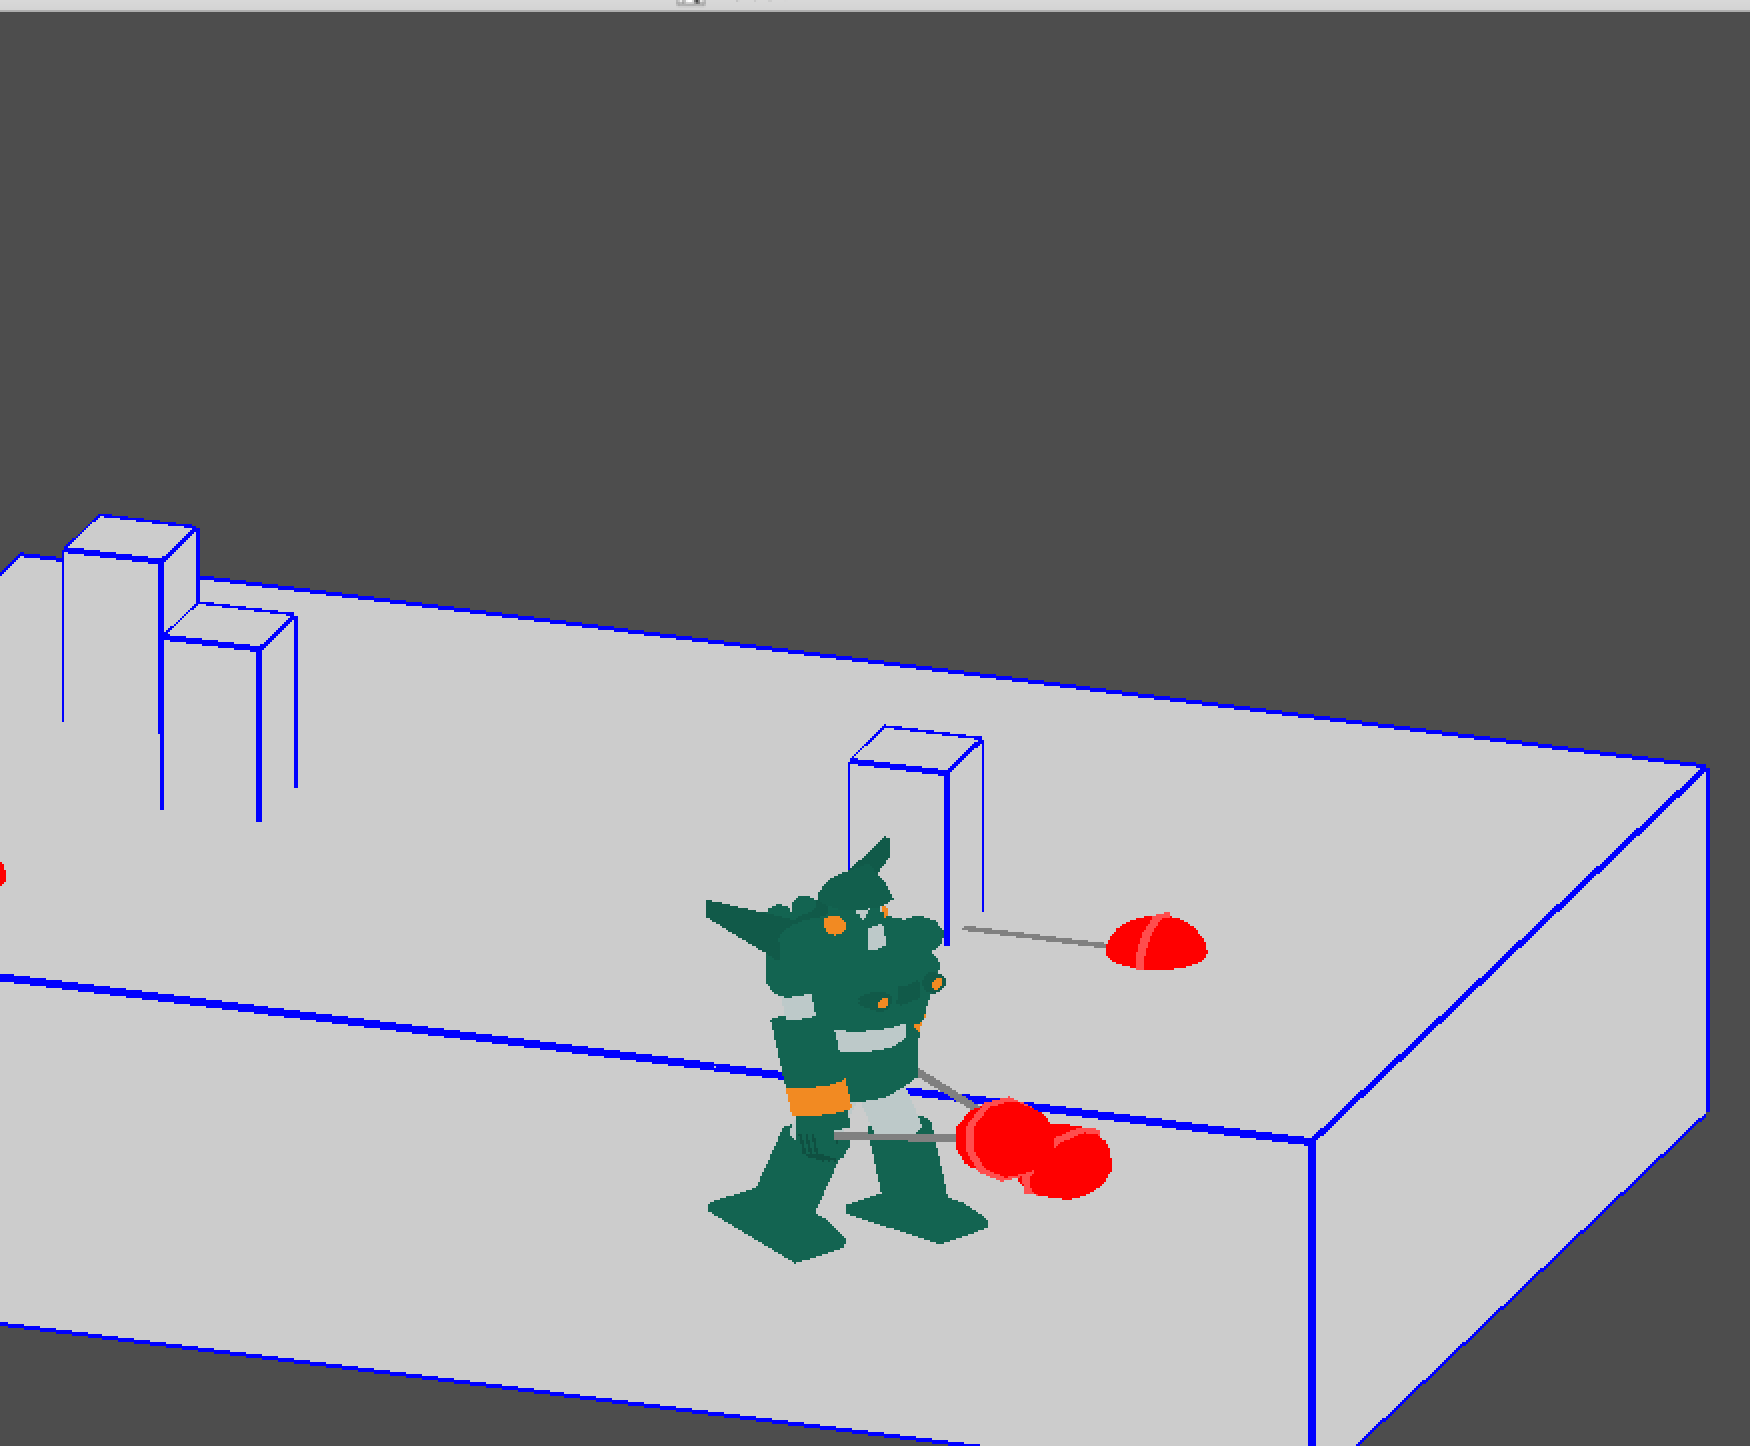
\includegraphics[scale = 0.3]{robot2.png}
    \caption{機器人2}
    \end{figure}
    
\end{document}